\documentclass[%
  paper=a4,
  twoside=false,				% two sided layout (=true) or one sided
  fontsize=13pt,
  DIV=12,
  BCOR=2mm,						% set binding correction width, i.e. width that is obscured by binding 
								%   method and has to be added on the inner side
  bibliography=totocnumbered,
  toc=listofnumbered,
  draft=false,
  captions=tableheading,
  abstract=on
]
{scrreprt}

\input{elements/preamble.header}
\input{elements/preamble.options}
%%%%%%%%%%%%%%%%%%%%%%%%%%%%%%%%%%%%%%%%%%%%%%%%%%%%%
%           Math hacks to simplify output           %
%                                                   %
%  Careful: Some hacks will ensure math mode        %
%      automatically, and thus can fail normal      %
%      expectations!                                %
%  Require package amsmath                          %
%%%%%%%%%%%%%%%%%%%%%%%%%%%%%%%%%%%%%%%%%%%%%%%%%%%%%
%% \bunderline
%%    An improved version of the underline command
%%
%%    Has one optional argument which defines how much
%%    the underline line is shortened. 
%%
%%    Example \underline[4]{<text>}
%%
%%    Source:
%%      http://tex.stackexchange.com/questions/49324/decrease-length-of-underline-in-math
\newcommand{\bunderline}[2][4]{\underline{#2\mkern-#1mu}\mkern#1mu}

%% \boverline
%%    An improved version of the overline command
%%
%%    Has one optional argument which defines how much
%%    the overline line is shortened
%%
%%    Source:
%%      http://tex.stackexchange.com/questions/22100/the-bar-and-overline-commands/22134#22134
\newcommand{\boverline}[2][1.5]{\mkern #1mu\overline{\mkern-#1mu#2\mkern-#1mu}\mkern #1mu}

%% \vect(or)
%%   Displays a variable as vector, can also be used
%%   in text environment. Three alternatives exist:
%%     - arrow vector notation
%%     - bold
%%     - underline
%%   Uncomment only the specific line to change format
%%   
%%   Careful: This command ensures math mode!
%%
%\newcommand{\vect}[1]{\ensuremath{\vec{#1}}}          % arrow
\newcommand{\vect}[1]{\ensuremath{\boldsymbol{#1}}}    % bold
%\newcommand{\vect}[1]{\ensuremath{\bunderline{#1}}}    % underline

%% \tensor
%%   Displays a variable as a tensor
%%   
%%   Careful: This command ensures math mode!
%%
%\newcommand{\tensor}[1]{\ensuremath{\boldsymbol{#1}}}            % bold
\newcommand{\tensor}[1]{\ensuremath{\bunderline{\boldsymbol{#1}}}} % bold underlined

%% \div, \Div
%%   Displays the mathematical operator of divergence.
%%   Faciliates brackets in capital version.
%%   Optional arguments
%%    #1 Type of parentheses
%%      Has no influence in \div version
%%      [square || <else>=round ]
%%
%%   Example: \Div[square]{\rho \vec{u}}
%%            \div{\vec{u}}
%%
%%   Careful: Overwrites the original div command!
%%
\renewcommand{\div}[2][1=round]{\nabla \cdot #2}
\newcommandx{\Div}[2][1=round]{%
  \ifthenelse{\equal{#1}{square}}{%
    % use square brackets
    \nabla \cdot \left[ #2 \right]
  }{%
    % use round braces
    \nabla \cdot \left( #2 \right)
  }
}

%% \grad, \Grad
%%    Displays the mathimatical operator of a gradient
%%    Faciliates brackets in captial version
\newcommand{\grad}[2][1=irrelevant]{\nabla #2}
\newcommandx{\Grad}[2][1=round]{%
  \ifthenelse{\equal{#1}{square}}{%
    % use square brackets
    \nabla \left[ #2 \right]
  }{%
    % use round braces
    \nabla \left( #2 \right)
  }
}

%% \mt
%%   Shortcut to insert text in math mode that is
%%   printed italic to mimic math font, but more 
%%   dense than normal math output.
\newcommand{\mt}[1]{\ensuremath{\text{\textit{#1}}}}

%% \parder, \Parder
%%    Displays a partial derivative
%%    Arguments:
%%      #2 Numerator
%%      #3 Demunerator
%%    Optional arguments:
%%      #1 Type of parantheses. Has no influence
%%        lower case version \parder
%%        'square' version will move the numerator
%%        after the fraction
%%        [square || <else>=round ]
%%
%%    Example: \parder{\vec{u}}{t}
%%             \Parder{\rho \vec{u}}{t}
%%             \Parder[square]{\rho \left( e + \frac{\vec{v}^2}{2}\right)}{t}
%%
\newcommand{\parder}[3][1=irrelevant]{\frac{\partial #2}{\partial #3}}
\newcommand{\Parder}[3][1=square]{
  \ifthenelse{\equal{#1}{square}}{
    \frac{\partial}{\partial #3} \left[ #2 \right]
  }{
    \frac{\partial \left(#2\right)}{\partial #3}
  }
}

%% \der, \Der
%%    Simple derivative
%%    Same options as \parder, \Parder
%%    but uses 'd' as derivative term instead of '\partial' (=delta)
\newcommand{\der}[3][1=irrelevant]{\frac{\mathrm{d}#1}{\mathrm{d}#2}}
\newcommand{\Der}[3][1=square]{
  \ifthenelse{\equal{#1}{square}}{
    \frac{\mathrm{d}}{\mathrm{d} #3} \left[ #2 \right]
  }{
    \frac{\mathrm{d} \left(#2\right)}{\mathrm{d} #3}
  }
}

%% \e
%%    Shortcut for printing 10^x coefficients
%%
%%    Example:  5\e{-3} -> 5*10^(-3)
%%
\newcommand{\e}[1]{\ensuremath{\cdot 10^{#1}}}

%% \exp
%%    Shortcut for the e^x notations
%%
%%  Example:    \exp{3} -> e^3
%%
\renewcommand{\exp}[1]{\mathrm{e}^{#1}}

%% \OD
%%    Shortcut for printing an OD
\newcommand{\OD}[2][1=750]{%
    \ensuremath{%
        % if #2 is empty just print OD_#1
        %   otherwise add the value
        \ifthenelse{\equal{#2}{}}{%
            \mathrm{OD}_{#1}%
        }{%
            \mathrm{OD}_{#1} = #2%
        }%
    }%
}

\DeclareMathOperator{\Var}{Var}

%% \transpose, \Transpose
%%    Shortcut to mark a matrix/tensor as transposed
%%    Uses the below defined \transposeSymbol
%%
%%    The uppercase variant checks for an optional first 
%%    parameter, which can either be "round" or "square"
%%    and will print parentheses or brackets around the 
%%    text.
%%
%%  Example:    \transpose{\tensor{\tau}}
%%              \Transpose[square]{\tensor{\tau}}
%%
\def\transposeSymbol{\intercal}
\newcommand{\transpose}[2][1=irrelevant]{\ensuremath{#2^\transposeSymbol}}
\newcommandx{\Transpose}[2][1=round]{%
  \ifthenelse{\equal{#1}{square}}{
    \ensuremath{\left[#2\right]^\transposeSymbol}
  }{%
    \ensuremath{\left(#2\right)^\transposeSymbol}
  }
}

\newcommand{\registered}{\textsuperscript{\textregistered}}

% the starred version of \ref will not create a link,
% but this fails anyway for all externalised images
\newcommand{\plotref}[1]{\tikzexternaldisable\ref*{#1}\tikzexternalenable}

\newcommand{\inlinetikz}[2][baseline=0]{%
  \tikzset{external/export next=false}%
  \tikz[#1]{#2}%
}

\newcommand{\imagelegend}[2][1=style]{%
  \ifthenelse{\equal{#1}{line}}{
    % #1 = line
    \inlinetikz{\draw [#2] (0, .25\baselineskip) -- (0.6, .25\baselineskip);}%
  }{
    % #1 = style
    \inlinetikz{\node [minimum size=0.5\baselineskip, #2, inner sep=0.1] at (0, 0.25\baselineskip) {};}%
  }
}

%% new the command for externalised tikz filenames
\newcommandx{\tikzsetnextfilenamecoloured}[2][1=colour]{%
  \ifthenelse{\equal{#1}{colour}}{
    % add a suffix tu determine wheter the graphic is colored or black and white
    \tikzsetnextfilename{#2\tikzExternalSuffix}
  }{
    \tikzsetnextfilename{#2}
  }
}

\pgfplotsset{ignore legend/.style={every axis legend/.code={
    \renewcommand\addlegendentry[2][]{} 
    \renewcommand\addlegendentryexpanded[2][]{}
    }}}

% \tablefootnote
%   This command can be used to manually create footnotes in a table
%   where it defines required extra spaces.
%   ! No automation at all
%
%   Use this command the following way:
%       Add "\textsuperscript{(2)}" in the table to reference footnote (2)
%           of the table below
%       Put the following code below the table to explain the footnotes 
%           you added
%
%           \tablefootnote{
%               \raggedright
%               \begin{tabular}{ll}
%               \multirow{3}{0.5cm}{} & \textsuperscript{(1)}Footnotetext 1 \tabularnewline
%                                     & \textsuperscript{(2)}Footnotetext 2 \tabularnewline
%                                     & \textsuperscript{(3)}Footnotetext 3
%               \end{tabular}
%           }
%       Adjust the number of multiple rows to the number of footnotes you 
%           have inserted. Furthermore you can manually adjust the space 
%           the first column takes up to center the footnotes
\newcommand{\tablefootnote}[1]{
    \vskip+\abovecaptionskip 
    \vskip-\belowcaptionskip
    \caption*{#1}
    \vskip-\abovecaptionskip
    \vskip+\belowcaptionskip
  }
  
\newcommand{\pictureheadnote}[1]{
    \vskip-\abovecaptionskip 
    \vskip+\belowcaptionskip
    \caption*{#1}
    %\vskip+\abovecaptionskip
    \vskip-\belowcaptionskip
  }
  
\let\originalparagraph\paragraph
\renewcommand{\paragraph}[2][.]{\originalparagraph{#2#1}}

% style to only print last n rows
\pgfkeys{
    /pgfplots/table/print last/.style={
        row predicate/.code={
            % Calculate where to start printing, use `truncatemacro` to get an integer without .0
            \pgfmathtruncatemacro\firstprintedrownumber{\pgfplotstablerows-#1} 
            \ifnum##1<\firstprintedrownumber\relax
                \pgfplotstableuserowfalse
            \fi
        }
    },
    /pgfplots/table/print last/.default=1
}

\pgfplotsset{
    simulation-plot/.style = {
        each nth point=10, filter discard warning=false,
        mark=none,
        x=Time,
        thick,
    },
    measurements-plot/.style = {
        mark=*, only marks, mark size=2pt, mark options={},
        x=Time,
        forget plot,
        error bars/y dir=both, error bars/y fixed relative=0.05,
    },
}

% pgfplots / pgfplotstable styles to filter tabledata,
% both copied from
% tex.stackexchange.com/questions/98003/filter-rows-from-a-table

\makeatletter
\pgfplotstableset{
    discard if not/.style 2 args={
        row predicate/.code={
            \def\pgfplotstable@loc@TMPd{\pgfplotstablegetelem{##1}{#1}\of}
            \expandafter\pgfplotstable@loc@TMPd\pgfplotstablename
            \edef\tempa{\pgfplotsretval}
            \edef\tempb{#2}
            \ifx\tempa\tempb
            \else
                \pgfplotstableuserowfalse
            \fi
        }
    }
}
\makeatother
    
\pgfplotsset{
    discard if not/.style 2 args={
    	x filter/.code={
    	    \edef\tempa{\thisrow{#1}}
    	    \edef\tempb{#2}
    	    \ifx\tempa\tempb
    	    \else
    	    \def\pgfmathresult{inf}
    	    \fi
    	}
    }
}

\usepackage[novbox]{pdfsync}

% arguments:
%   1: [order] (l, r, p, p!)
%   2: text
%   3: [width] ... of textbox
%   4: [spacing] ... between boxes
%   5: picture
\newlength{\picboxwidth}
\newcommandx{\besidespic}[5][1=p, 3=0.65\textwidth, 4=0.05\textwidth]{%
  {
  % need to put this in a local environment, otherwise values will be assigned globally
  \setlength{\picboxwidth}{\textwidth}
  \addtolength{\picboxwidth}{-#3}
  \addtolength{\picboxwidth}{-#4}
  \captionsetup{format=plain}
  
  % evaluate special cases position=p or p!
  %   set \pic to contain picture position
  \ifthenelse{\equal{#1}{p}}{
    % option p
    % notcomascript-documents
    %\ifthenelse{\isodd{\thepage}}{
    % Koma Script based documents
    \ifthispageodd{
      % odd
      \def\pic{r}
    }{
      % even
      \def\pic{l}
    }
  }{
    \ifthenelse{\equal{#1}{p!}}{
      % option p!
      % notcomascript-documents
      %\ifthenelse{\isodd{\thepage}}{
      % Koma Script based documents
      \ifthispageodd{
        % odd
        \def\pic{l}
      }{
        % even
        \def\pic{r}
      }
    }{
      \def\pic{#1}
    }
  }
  
  %% Output text and picture
  \ifthenelse{\equal{\pic}{l}}{
    \begin{minipage}[c]{\picboxwidth}
      #5
    \end{minipage}\hspace{#4}
    \begin{minipage}[c]{#3}
      #2
    \end{minipage}
  }{
    \begin{minipage}[c]{#3}
      #2
    \end{minipage}\hspace{#4}
    \begin{minipage}[c]{\picboxwidth}
      #5
    \end{minipage}
  }
  
  % end of seperate environment
  }
}

%%%%%%%%%%%%%%%%%%%%%%%%%%%%%%%%%%%%%%%%%%%%%%%%%%%%%
% Bibliography use brackets [] instead of braces () %
%%%%%%%%%%%%%%%%%%%%%%%%%%%%%%%%%%%%%%%%%%%%%%%%%%%%%
\makeatletter

\newrobustcmd*{\parentexttrack}[1]{%
  \begingroup
  \blx@blxinit
  \blx@setsfcodes
  \blx@bibopenparen#1\blx@bibcloseparen
  \endgroup}

\AtEveryCite{%
  \let\parentext=\parentexttrack%
  \let\bibopenparen=\bibopenbracket%
  \let\bibcloseparen=\bibclosebracket}

\makeatother

\DeclareCiteCommand{\citetitlelink}
  {\boolfalse{citetracker}%
   \boolfalse{pagetracker}%
   \usebibmacro{prenote}}
  {\ifciteindex
     {\indexfield{indextitle}}
     {}%
   \printtext[bibhyperref]{\printfield[citetitle]{labeltitle}}}
  {\multicitedelim}
  {\usebibmacro{postnote}}

%%%%%%%%%%%%%%%%%%%%%%%%%%%%%%%%%%%%%%%%%%%%%%%%%%%%%
% Shortcuts for company names with registered char  %
%%%%%%%%%%%%%%%%%%%%%%%%%%%%%%%%%%%%%%%%%%%%%%%%%%%%%
% print ANSYS Fluent name with registered trademark symbol
\newcommand{\fluent}{ANSYS\textsuperscript{\textregistered} Fluent\textsuperscript{\textregistered}}
% print ANSYS ICEM name with registered trademark
\newcommand{\icem}{ANSYS\textsuperscript{\textregistered} ICEM\textsuperscript{\textregistered}}
% print OpenFOAM with registered trademark symbol
\newcommand{\openfoam}{OpenFOAM\textsuperscript{\textregistered}}
% print ansys without a specific product
\newcommand{\ansys}{ANSYS\textsuperscript{\textregistered}}
% print Matlab with registered trademark symbol
\newcommand{\matlab}{MATLAB\textsuperscript{\textregistered}}

%%%%%%%%%%%%%%%%%%%%%%%%%%%%%%%%%%%%%%%%%%%%%%%%%%%%%
%    Have abbreviation shortcuts to avoid end of    %
%             sentence spacing problems             %
%%%%%%%%%%%%%%%%%%%%%%%%%%%%%%%%%%%%%%%%%%%%%%%%%%%%%
\makeatletter
\newcommand{\etc}{etc\@ifnextchar.{}{.\@}}      % etc.
\newcommand{\eg}{e.g\@ifnextchar.{}{.\@}}       % e.g.
\newcommand{\ie}{i.e\@ifnextchar.{}{.\@}}       % i.e.
\makeatother

%%%%%%%%%%%%%%%%%%%%%%%%%%%%%%%%%%%%%%%%%%%%%%%%%%%%%
%        Declare special unicode characters         %
%%%%%%%%%%%%%%%%%%%%%%%%%%%%%%%%%%%%%%%%%%%%%%%%%%%%%
%\DeclareUnicodeCharacter{010C}{\v{C}}  % Č

\widowpenalty10000
\clubpenalty10000
\input{elements/preamble.tikzit}

\begin{document}

% Keine Kopf-/Fusszeilen auf den ersten Seiten.
\pagestyle{empty} 

% Title page
\begin{figure}[H]
	\begin{center}
		\includegraphics[width=0.15\textwidth]{images/title/logo-TUM-empty}
    \hspace{.65\textwidth}
    
\includegraphics[width=0.15\textwidth]{images/title/logo-MW}
	\end{center}
\end{figure}
%\vspace{5mm}

\begin{center}
	{\Huge Technische Universit\"at M\"unchen}
	\\[5mm]
	{\Large Lehrstuhl f\"ur Bioverfahrenstechnik}
\end{center}

\vspace{15mm}

\begin{center}
    \begin{minipage}{.7\textwidth}
        \begin{center}
            \doublespacing
            {
                {
                    \Large Semesterarbeit
                    %\Large Masterarbeit
                }
                \\[1cm]
                \textbf{\LARGE Development of a Low-Cost Electrical Conductivity Meter for Liquids}
            }
            \\[3.5cm]
            {\Large Sebastian Plamauer}
            \\
            {\normalsize Matrikelnummer: 3609702}
            \\[0.5cm]
            \today
        \end{center}
    \end{minipage}
\end{center}

\vspace{\fill}
  
\begin{center}
    \begin{tabular}{p{3cm}l}
        Betreuer: & M.Sc. Timm Severin \\
        & Prof.~Dr.-Ing.~Dirk~Weuster-Botz
    \end{tabular}	 
\end{center}

% Empty page after title
\clearpage\mbox{}\clearpage

%% Sentence for fun
%\newpage
%\null \vfill
%\textit{So Long, and Thanks for All the Fish}
%
%\hspace{1cm} [Douglas Adams, 1984]

\include{elements/declaration-of-authorship}

% Page design (Header, Footer)
\setheadwidth{\textwidth}
\ohead{\pagemark}
\chead{} \cfoot{} \ofoot{} \ifoot{}
\ihead{\sffamily \leftmark}
\pagestyle{scrheadings}

%% Tikz Testarea BEGIN
%\begin{figure}[H]%
  %\centering
  %%\caption{}%
  %%\label{}%
%\end{figure}
%% Tikz Testarea END

\begin{abstract}

In the light of problems surrounding the use of fossil fuels, photobioreactors emerge as a cost effective option to produce climate-neutral and renewable bio-fuels. To study and improve those reactors simulations and experiments are necessary. To enable the measurement and analysis of the flow in the reactor this thesis develops a low-cost electrical conductivity meter to measure changes of salinity in a flowing liquid. This allows for tracking saltwater pulses in a freshwater flow, indicating the movement of the volumes. The resulting system was successfully tested and generated usable data.

\end{abstract}

\tableofcontents

\chapter{Introduction}

Fossil fuels play a large role in the world's energy production and as energy sources for transportation vehicles. Especially for vehicles, their high energy density and liquid form at room temperature has enabled the construction and operation of cars and airplanes otherwise not possible.
At the same time, there are fundamental problems in using fossil fuels as energy sources. Be it oil, coal or gas, the formation of these resources is a natural process spanning millions of years. This means that once the current reserves are depleted, they will not be refilled. Even without depleting all the reserves, the depletion of the easily reachable reserves means that ever greater effort has to be taken to find and use less accessible fields, using methods with severe impact on the environment.
In addition to that, burning fossil fuels for energy also releases a slew of gases into the atmosphere, of which CO2 is the most prominent. CO2 is a greenhouse gas and as such influences the worlds climate tremendously.

In light of those problems, renewable energy sources are needed. For electricity production there are a some attractive technologies already in use that directly or indirectly generate power using the sun. For vehicles, using electrical power can be problematic. The electricity has to be stored in batteries, and even with the higher efficiency of electrical motors, the lowered energy density reduces range drastically. Batteries also have to be charged, as opposed to be refilled like tanks, which takes substantially more time. While for some vehicles, like cars, this technology still can be made feasible, it is much less suitable for airplanes.

For these applications a more direct replacement for fossil fuels has to be found. A possible solution are bio-fuels. Bio-fuels are generated from biomass, for example plants. An important requirement for the growth of biomass in order to produce bio-fuel is to avoid competition over land and resources with food production. A low price is also important to make the product economically viable.

One technology which potentially fits these needs are open photobioreactors (PBR) growing microalgae. These algae produce lipids, which can be processed to fuel. To improve and optimize these reactors experiments and models are needed. A computational fluid dynamics (CFD) simulation models the flow in the reactor. In order to validate this simulation, experiments measuring the flow conditions in the reactor have to be conducted. To do so, a sensor system needs to be developed. The option explored in this thesis is to measure the stream's conductivity. The next chapter will describe the objectives and criteria of this system in detail.
\chapter{Objectives} \label{obj}

The goal of this project is the development and test of a low-cost electrical conductivity meter for liquids to be used as an aid to measure and analyze the flow in photobioreactors like the one depicted in Figure \ref{fig:pbr}.

\begin{figure}
	\begin{center}
	\tikzset{external/export next=false}
	\begin{tikzpicture}
		\node[,inner sep=0] at (0,0) {\includegraphics[width=\textwidth]{images/pbr.jpg}};
		\draw[red!80!blue,ultra thick] (-5,1.5) ellipse (1.75 and 1.25);
		\draw[green!80!blue,ultra thick] (-2,-2) ellipse (3.25 and 2.25);
		\draw[-latex, blue!80!white, ultra thick] (-0.9,1.1) -- (2,1.15);
		\draw[-latex, blue!80!white, ultra thick] (2.25,-0.45) -- (0.85,-0.8);
		\draw[-latex, blue!80!white, ultra thick] (4.5,1) .. controls (5,0.75) and (4.5,0) ..  (3.75,-0.15);
	\end{tikzpicture}
		\caption[The photobioreactor for which the conductivity meter is developed]{The photobioreactor for which the conductivity meter is developed - Water enters through the inlet basin, (\drawline[red!80!blue]), streams down the ramp (\drawline[blue!80!white,-latex]) to the collection tank (\drawline[green!80!blue]) from where it is pumped back to the inlet.}
		\label{fig:pbr}
	\end{center}
\end{figure}

The method chosen beforehand is to measure the fluids' electrical conductivity, which can be changed easily by adding water with differing salt concentrations. The conductivity increases for higher salinities and decreases for lower ones. By adding a saltwater impulse upstream, the changes in salinity downstream can be measured and used to gather information about the behavior of the stream.

Commercially available conductivity meters are built to measure with high accuracy in order to obtain information about a liquid's absolute salinity and are relatively expensive. In our case, however, the meter does not need to create high-accuracy absolute measurements, but measure a relative change allowing to distinguish different liquids by their salinity. However, this needs to happen very fast and at a lot of different points in the stream. The more positions measured, the more complete the picture of the flow becomes. Therefore, the cost per sensor has to be low, to not put a restraint on the total number of points that can be measured.

The actual flow analysis is not the focus of this work, but rather the creation of a tool to make it possible. As such, the system needs to be designed to be easily usable by people without deep knowledge of the underlying technology.\\

The following sections describe and detail the requirements the sensor system has to fulfill in order to meet the objectives. These requirements translate the objectives into discrete and verifiable units, serving as the base for development and benchmark for the later performance analysis. 

\section{Spacial and Time Resolution}

The spacial resolution $ \diff s $ and the time resolution $ \diff t $ decide the granularity of the flow image. Both resolutions are connected by the velocity $ v $ of the stream flowing over the sensor as shown in equation \eqref{eq:resv}.

\begin{equation}
	v = \dfrac{\diff s}{\diff t}
\label{eq:resv} 
\end{equation}

With both resolutions connected, only one of them has to be defined. \\

The information gathered by the sensor has to be granular enough to enable the verification of the simulation. As it is not possible to derive a hard number from that, the following list shows different deliberations to establish a first estimate. \\

\begin{itemize}
\item The granularity of the simulation is determined by its mesh size and is in the order of about 1 to \unit[5]{mm}. A resolution better than that would be unnecessary, making this the upper limit.

\item The data collected by the sensor system shows the salinity of the liquid passing a certain position over time. By extracting the same data from the simulation, a graph can be compiled comparing the measured to the simulated values. The flow becomes visible when comparing data from different positions. The first sensor to show a spike in salinity is further up the stream than sensors spiking later. The distance between two sensors has to be big enough for a given velocity of the stream so that the time delay can be clearly seen. At a flow speed of $ v $ in the order of \unitfrac[1]{m}{s}, a resolution in the order of centimeters would yield time differences of centiseconds. Whether or not this is sufficient depends on noise and delay in the sensor system, however centiseconds is a conservative estimate likely to be achievable.

\item The geometry of the inlet basin of the bioreactor as shown in figure \ref{fig:elb} also influences the needed resolution. It has to be an order of magnitude smaller than the basins characteristic length, in this case the width of \unit[850]{mm}, to enable gathering data about the flow conditions within.
\end{itemize}

Derived from all that, a spacial resolution in the order of centimeters, is chosen as requirement.

\begin{figure}
	\begin{center}
		\includegraphics[width=\textwidth]{images/Einlaufbecken.pdf} 
		\caption[The inlet basin]{The inlet basin - water is fed back from the bottom of the reactor to the inlet.}
		\label{fig:elb}
	\end{center}
\end{figure}

\section{Electrical Conductivity Resolution}

To measure the change in conductivity of the water stream after changing it in the feed, the system has to be able to distinguish between water with different salinities. The water used normally in the reactor is tap water with a salinity of about \unit[0.2]{\%}. The salinity of the added saltwater can be chosen freely. Water with a salinity of about \unit[5]{\%} is easily available in the facilities and offers a sensible choice. Assuming a reactor with \unit[65]{l} in circulation and an added saltwater impulse of \unit[5]{l}, the resulting salinity after perfect homogenization would be approximately \unit[0.54]{\%}. The system has to be able to clearly distinguish between all those salinities. The sensors sensitivity therefore shall be better than a change of \unit[0.1]{\%} salinity with a range from 0 to \unit[5]{\%}.

\section{Cost}

The more sensors used, the more points in the stream can be measured and the better the resulting image of the stream. Therefore, the cost per sensor has to be low enough to not be prohibitive to adding more sensors.
The cost of a high quality lab conductivity meter is in the range of \euro{1000} and was set as the goal of maximum cost for the sensor system. The number of sensors needed to cover all interesting regions of the bioreactors is about 40.
A maximum cost of \euro{25} per sensor results from those figures.

\section{Usability}

The sensor system is meant to be used in the algae reactors of the algae cultivation center at the Ludwig Bölkow Campus. It should be possible to easily mount and remove the system to and from the reactor without having to dismantle the latter.

The system also has to be easy to use, so it can be helpful to the researchers working on the reactor. It has to work reliably and act according to expectations of the users. The risk of handling errors that lead to loss of data has to be minimized. All operations have to be documented in a minimal set of written instructions, so that the system can still be used even if the developer is not available.

\section{Summary of Requirements}

Table \ref{tab:req} concludes and displays all requirements alongside the methods of verification to be used.

\begin{table}[H]
    \centering

    \caption[Requirements]{Requirements}
    \label{tab:req}
    \begin{tabular}{lp{.7\textwidth}l}
        	\toprule
        	Nr. & Requirement & Verification \tabularnewline
        	\midrule
		1 & The system shall have a spacial resolution in the order of \unit[10]{mm}. & Test, Inspection \tabularnewline
		2 & The system shall have a sensitivity of  \unit[0.1]{\%} salinity.  & Test \tabularnewline
		3 & The system shall have a range from 0 to \unit[5]{\%} salinity.  & Test \tabularnewline
		4 & The cost per sensor shall be less than \euro{25}.  & Analysis \tabularnewline
		5 & The system shall be deployable in the algae reactor. & Demonstr. \tabularnewline
		6 & The system shall be usable with a set of written instructions. & Test, Review \tabularnewline
        \bottomrule
    \end{tabular}
\end{table}

\include{content/theory}

\chapter{Design}

This chapter describes the design of the sensor system and all components involved. The system consists of several parts playing different roles. The System Design gives an overview of these parts, their purpose and their communication with each other. Afterwards, these subsystem are described in detail.\\

\section{System Design}

On the user-facing side there is a personal computer (PC). This PC runs software that visualizes a live data stream and provides a control interface for the sensor system. It is connected via USB to a microcontroller. This microcontroller controls the MinieeC interface via I2C, reads the measurement data from it and sends it to the PC. It also controls the matrix switches. The MinieC Interface provides the signal and ground between which the resistance is measured. Both lines are connected to one matrix switch each. These matrix switches are able to connect one input to 8 different outputs. On each of those outputs, one electrode is connected. The matrix switches can thereby connect the MinieC interface to one of 8 electrode pairs. \\

Using the matrix switches, 8 electrodes can be used with just one MinieC interface. Increasing the number of electrodes can be done in two ways:

\begin{itemize}
    \item by chaining up multiple stages of matrix switches, the number of electrodes can be increased eightfold with each stage
    \item by connecting another MinieC Interface with it's own set of matrix switches to the microcontroller, 8 more electrodes can be added with each of these subsystems
\end{itemize}

The first option results in lower cost per added electrode, as the MinieC interface is reused. However, with a system like that, all electrodes have to be read in serial, while with the second option each MinieC interface can read in parallel, resulting in higher sample rate. Practically the second option is also easier to achieve. For the first option, a board with 18 matrix switches and 80 connections is needed, while the second option only uses 2 switches per board resulting in 16 connections. The simpler board greatly reduces complexity and can also be made smaller.

\begin{figure}
	\begin{center}
\begin{tikzpicture}
	\begin{pgfonlayer}{nodelayer}
		\node [rounded corners=8pt, inner sep=16pt, style=rect] (0) at (8, -1) {8 Electrodes};
		\node [rounded corners=8pt, inner sep=16pt, style=rect] (1) at (0, 3) {Microcontroller};
		\node [rounded corners=8pt, inner sep=16pt, style=rect] (2) at (-3, -1) {MinieC Interface};
		\node [rounded corners=8pt, inner sep=16pt, style=rect] (3) at (3, 0.25) {Matrix Switch};
		\node [rounded corners=8pt, inner sep=16pt, style=rect] (4) at (0, 6) {PC};
		\node [style=rect, inner sep=16pt, rounded corners=8pt] (5) at (3, -2.25) {Matrix Switch};
	\end{pgfonlayer}
	\begin{pgfonlayer}{edgelayer}
		\draw [style=darrow] (4) to node[left]{USB} (1);
		\draw [style=simple, bend right=15, looseness=1.00] (0) to node[above]{8 SIG} (3);
		\draw [style=simple, bend right=15, looseness=1.00] (3) to node[above]{SIG} (2);
		\draw [style=arrow, bend left=15, looseness=1.00] (1) to node[right]{SPI} (3);
		\draw [style=darrow, bend right=15, looseness=1.00] (1) to node[left]{I2C} (2);
		\draw [style=simple, bend right=15, looseness=1.00] (2) to node[below]{GND} (5);
		\draw [style=simple, bend right=15, looseness=1.00] (5) to node[below]{8 GND} (0);
		\draw [style=arrow, bend left=15, looseness=1.00] (1) to node[right, pos=0.9]{SPI} (5);
	\end{pgfonlayer}
		\draw (-5.5,-3.5) -- (10,-3.5) -- (10,2) node[below, left, yshift=-8pt] {$n$} -- (-5.5,2) -- (-5.5,-3.5);
\end{tikzpicture}
		%\input{images/system_design.tikz}
		%\includegraphics[width=\textwidth]{images/systemdesign.pdf} 
		\caption{System Design}
		\label{fig:sys}
	\end{center}
\end{figure}

\section{Electrodes}

The electrode pairs are the actual sensors in contact with the fluid to be measured. Their material and geometry influence the measuring range of the system. According to information in the book \cite{trankler2015sensortechnik} a cell constant $ C $ of $1$ enables a range from \unitfrac[$2 \cdot 10^3$]{$\mu S$}{cm} to \unitfrac[$10 \cdot 10^3$]{$\mu S$}{cm}. For a water temperature of \unit[$18^\circ$]{C} this corresponds to salinities of \unit[0.66]{\%} and \unit[0.12]{\%}. While this theoretical range is not sufficient for our purpose, first tests showed that the achievable range is much bigger than described in the book. The book doesn't specify the materials influence on the range and it also doesn't qualify how the usable range is defined. As our application has much lower demands on accuracy as the usual ones, this might be an explanation for the discrepancy. \\

Figure \ref{fig:sensor} shows the geometry of the sensor. To achieve a cell constant $C$ of $1$, a width $w$ of \unit[1]{mm}, height $h$ of \unit[10]{mm} and distance $d$ of \unit[10]{mm} were chosen.\\

\begin{figure}
	\begin{center}
		\begin{tikzpicture}
			\draw [line width=0.5mm] (-1,-1) -- (-1,1) -- (-1.3,1) -- (-1.3,-1) -- (-1,-1);
			\draw [dash dot] (-1.15,-1.5) -- (-1.15,1.2);
			\draw [line width=0.5mm] (1,-1) -- (1,1) -- (1.3,1) -- (1.3,-1) -- (1,-1);
			\draw [dash dot] (1.15,-1.5) -- (1.15,1.2);

			\draw (-1,1.6) -- (-1,1);
			\draw (-1.3,1.6) -- (-1.3,1);
			\draw (-1,1.4) -- (-1.3,1.4) node[above, pos=-0.75] {$w$};
			\draw [arrow]  (-1.7,1.4) -- (-1.3,1.4);
			\draw [arrow] (-0.6,1.4) -- (-1,1.4);
			
			\draw (-1.9,1) -- (-1.3,1);
			\draw (-1.9,-1) -- (-1.3,-1);
			\draw [darrow] (-1.7,1) -- (-1.7,-1) node[left, pos=0.5] {$h$};

			\draw [darrow] (-1.15,-1.3) -- (1.15,-1.3) node[above, pos=0.5] {$d$};

		\end{tikzpicture}
		\caption{Electrode pair forming a sensor}
		\label{fig:sensor}
	\end{center}
\end{figure}

As a first proof-of-concept a the sensor was built as a sensor array, containing multiple electrode pairs on a strip \ref{fig:v2}. A \unit[5]{cm} wide and \unit[25]{cm} long band of Kapton adhesive tape served as the base. 4 electrode pairs made from \unit[0.2]{mm} platinum wire were arranged equidistant on the strip. \unit[0.4]{mm} enameled copper wire runs along the tape to connect each electrode pair to the left end of the strip, from which insulated cables run to the sensor node. After soldering the joints, two smaller strips of tape were used to cover the wiring, exposing only the electrodes to fluid.

First tests with this sensor array showed the viability of the concept, however a simple look at it shows the inherit problems. Instead of a uniformly flat strip with minimal influence on the flow, the assembly forms several irregularities. Soldering \unit[0.2]{mm} platinum wire to \unit[0.4]{mm} enameled copper wire on a piece of adhesive tape per hand also did not result in clean solder joints. And while with the experience of the first array, the second array turned out a bit cleaner, the fundamental problem remains: it is a tedious manufacturing process resulting in a low quality product.

\begin{figure}
	\begin{center}
		\includegraphics[width=\textwidth]{images/v2.jpg} 
		\caption{Handmade Sensor Strip}
		\label{fig:v2}
	\end{center}
\end{figure}

As an alternative to these handmade strips, industrially produced Flex-PCBs were identified. Flex-PCBs are flexible printed circuit boards that are very close to the handmade arrays described above. They also use Kapton as base, on which a copper coating gets applied and partially removed by etching to form the conducting paths. On top, another layer of Kapton is applied, with cutouts in the places where the copper is supposed to be exposed. The exposed copper is then plated with ENIG (Electroless nickel immersion gold) to protect the copper from oxidation and provide the landing pads for electrical components to be soldered on.

For our purpose those exposed and plated landing pads can be used as electrodes, being nicely embedded in a FlexPCB that also runs the wiring up to an interface from where cables can be run. Using the FlexPCB itself as cable is not viable due to the high cost per area.

The cables are soldered directly to the PCB and silicone is used to create a waterproof seal around the connection.

\begin{figure}
	\begin{center}
		\includegraphics[width=\textwidth]{images/fpcbd.pdf} 
		\caption{Design of FlexPCB}
		\label{fig:fpcbd}
	\end{center}
\end{figure}

\section{Matrix Switches}

The matrix switches are an essential part of the system, enabling it use multiple sensors with a single MinieC Interface, thus lowering the cost per sensor. The part used is an ADG738 from Analog Devices. It is an 8-channel CMOS analog matrix switch controlled via a 3-wire serial interface. The following information is taken from the data sheet \cite{ms}.\\

Figure \ref{fig:ms} shows the functional block diagram. The switch has one drain pin (D) and 8 source pins (S1..S8). Despite the naming of drain and source, the internals provide simple switches between the drain and each source pin. The switches work in both directions without any restriction on the signal beyond a maximum current of \unit[120]{mA} that far exceeds our needs. By sending control commands via the 3-wire interface, each of the 8 internal switches can be turned on and off individually.\\

\begin{figure}
	\begin{center}
		\includegraphics[width=0.3\textwidth]{images/ms.pdf} 
		\caption{Functional block diagram of ADG738}
		\label{fig:ms}
	\end{center}
\end{figure}

The example timing diagram \ref{fig:msc} describes the data transmission process. The microcontroller sends one byte of data to the matrix switch. Each of the 8 bits of this byte controls one switch. The first bit controls the first switch and so on. If the bit is 1, the switch is closed, if 0, the switch is open. To send the byte, first the synchronization pin (SYNC) has to be pulled low from it's usual high level. A clock signal is provided to the clock pin (SCLK). At each falling edge of the clock signal, the data input (DIN) is read - where high leads to a 1-bit and low to a zero-bit. After 8 cycles, SYNC is pulled high again marking the end of data transmission with a full byte transferred. After that, the switches immediately take their instructed states with switching times in the order of \unit[100]{ns}. In the example shown, the first switch is on, while all others are off.\\

\begin{figure}
	\begin{center}
	\tikzexternaldisable
		\begin{tikztimingtable}
  			SYNC   & H 32{L} H \\
  			SCLK   & C 16{2C} N(A1) C \\
  			DIN  	& 2{L} {2H} N(B1) 15{2L} \\
  			Data	& 2D{} 2D{1} 2D{} 2D{0} 2D{} 2D{0} 2D{} 2D{0} 2D{} 2D{0} 2D{} 2D{0} 2D{} 2D{0} 2D{} 2D{0} 2D{}\\
		\end{tikztimingtable}
		\caption{Timing diagram}
		\label{fig:msc}
	\end{center}
\end{figure}

Multiple matrix switches can be controlled at once by daisy-chaining the data output pin (DOUT) of the first device to DIN of the second one, and on so forth. Both SYNC and SCLK are connected to the same bus. This assures that all matrix switches are set in the same state and at the same time.

\section{MinieC Interface}

The sensor node logically consists of the signal generator and the signal reader, practically both parts are tightly integrated.

[Describe mini-eC-Interface]
[also where i.e. the change with the filter cap and the tests that surfaced the issue is described]

The mini-eC-Interface provides two channels to connect to the electrodes, but  multiple sensors should be driven by one interface. The method to this is called demultiplexing and the component able to this is the Matrix-Switch.
A Matrix-Switch is an electrical component containing a multitude of switches, where the switches can be electronically closed and opened from a controller. The Matrix-Switch chosen consists of 8 switches, where all switches have the same input, but separate outputs. Thus, they allow applying an input signal to different outputs. The input in our case is the signal and reference from the minie-eC-Interface, applied to 8 different electrode pairs making up the sensors. A separate Matrix-Switch is need for signal and reference.

\section{Microcontroller}

The Data Processing Unit has to be able to control the functions of the sensor nodes attached to it, read the data from them, log it and serve it to the user-interface. Typically, any micro-controller is is fit for those tasks. Micro-controllers usually are programmed in C or C++, however nowadays there are other options, too. One of those is Micropython, which is an implementation of the Python 3 programming language designed to run on micro-controllers. Python is a vastly easier language than C/C++, and this is especially true when the involved persons are not from a computer science or electrical engineering background, but i.e. mechanical engineering or other sciences. In those fields, Python is often familiar from usage for data processing and visualization. Using Micropython enables us to design a system where it is more likely that the people using it are able to understand the code, enabling them to improve it and adapt it to alternate use-cases.
It does however limit our choice of Hardware to supported platforms and it requires more powerful and thereby expensive micro-controllers. But as the system only requires one Data Processing unit to drive a very large amount of sensors, the added cost is relative and outweighed by the benefits of the better usability. While the factor of the expensive controllers to cheaper ones is about 10, the cost in the end is still only about \euro{7}.
For prototyping, a development board named "Espruino Pico" was chosen. It is a very small and simple board that provides the electrical boilerplate to use a micro-controller without needing to deal with the lowest level of electronics, like cleaning power supply, etc.

\section{User-Interface}
\chapter{Results}

\section{Verification}

Test for each requirement.

\subsection{Time Resolution}

Test if smaller then \unit[1]{ms}.

\subsection{Spacial Resolution}

Inspect if smaller then \unit[1]{cm}. [physical size of sensor is 1 cm, sensor can be directly next to each other. show via drawing]

\subsection{Electrical Conductivity Resolution}

Test if able to distinguish liquids with a conductivity of \unitfrac[5]{S}{m} and \unitfrac[5e-3]{S}{m}.

\subsection{Cost}

Analyse if less than \euro{10} per sensor.

\subsection{Deployment}

Demonstrate that deployable in the algae reactor.

\subsection{Usability}

Test if easy to use by anybody with only a minimal set of written instructions. [find a victim to try to perform a measurement with only written instructions provided]

\section{Validation}

Check, if Timm can use it to measure flow and compare with simulation. [?]

\begin{figure}
	\begin{center}
		\includegraphics[width=\textwidth]{images/noise.pdf} 
		\caption{noise}
	\end{center}
\end{figure}

\begin{figure}
	\begin{center}
		\includegraphics[width=\textwidth]{images/feed_switch.pdf} 
		\caption{feed switch}
	\end{center}
\end{figure}

\begin{figure}
	\begin{center}
		\includegraphics[width=\textwidth]{images/feed_add.pdf} 
		\caption{feed add}
	\end{center}
\end{figure}

\begin{figure}
	\begin{center}
		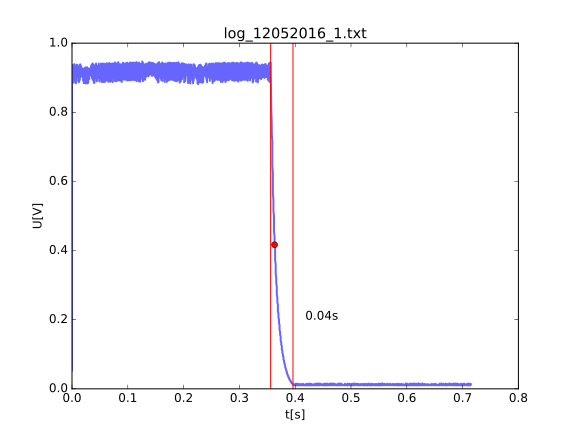
\includegraphics[width=\textwidth]{images/switch_cap.pdf} 
		\caption{switch cap}
	\end{center}
\end{figure}

\begin{figure}
	\begin{center}
		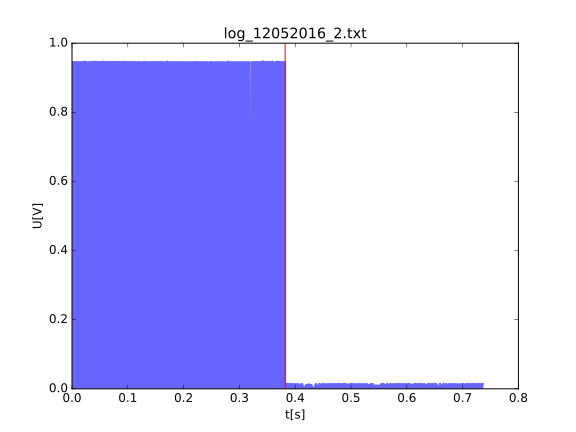
\includegraphics[width=\textwidth]{images/switch_nocap.pdf} 
		\caption{switch no cap}
	\end{center}
\end{figure}


\chapter{Conclusion}

The conclusion is it works.

%\include{content/examples}

%% Appendix
\appendix
                        % Appendix headline
\chapter{Appendix} 

\section{Instruction Manual} \label{aman}

\subsection*{Setting up the Hardware}

\begin{figure}[H]
	\begin{center}
		\tikzset{external/export next=false}
		\begin{tikzpicture}
			\node[,inner sep=0] at (0,0) {\includegraphics[width=0.5\textwidth]{images/cb.jpg}};
			\node[inner sep=0] at (0,-3) {\includegraphics[width=\textwidth]{images/fpcbp.jpg}};
			
			\draw[red,ultra thick,rounded corners] (-4,-0.55) rectangle (-3.25,0.55);
			
			%\draw[red!50!yellow,ultra thick,rounded corners] (-1,-0.35) rectangle (-0.25,0.35);
			%\draw[red!50!yellow,ultra thick,rounded corners] (0.55,-0.35) rectangle (1.3,0.35);
			
			\draw[red!25!yellow,ultra thick,rounded corners] (-1.45,-1) rectangle (-0.3,-0.6);
			\draw[red!25!yellow,ultra thick,rounded corners] (0.3,-1.05) rectangle (1.3,-0.65);
			\draw[red!25!yellow,ultra thick,rounded corners] (-1.54,1.05) rectangle (-0.44,0.65);
			\draw[red!25!yellow,ultra thick,rounded corners] (0.15,1.05) rectangle (1.15,0.65);
			
			%\draw[blue,ultra thick,rounded corners] (1.8,-1.2) rectangle (4,1.2);
			\draw[blue!75!white,ultra thick,rounded corners] (-8,-4) rectangle (8,-2);
			%\draw[blue!50!white,ultra thick,rounded corners] (-2.75,-3.5) rectangle (-1.65,-2.5);
		\end{tikzpicture}
		\caption[Important parts of the system.]{Important parts of the system:\\USB connection (\drawline[red,ultra thick])\\sensor strip (\drawline[blue!75!white,ultra thick])\\connectors (\drawline[red!25!yellow,ultra thick])}
		\label{fig:isysa}
	\end{center}
\end{figure}

\begin{itemize}
	\item[1] Use electrical tape to mount the sensor strips at desired points of measurement. Make sure not to cover the electrodes (golden parts).
	\item[2] Connect the cables of the sensor strip to the carrier board as shown in the picture:
	\begin{figure}[H]
	\begin{center}
		\includegraphics[width=0.5\textwidth]{images/conn.jpg}
		\caption{The connectors for the sensor strips.}
		\label{fig:iconna}
	\end{center}
\end{figure}
	\item[3] Connect the carrier board to the host PC with the USB cable. Note the orientation in the picture:
		\begin{figure}[H]
	\begin{center}
		\includegraphics[width=0.5\textwidth]{images/usb.jpg}
		\caption{The correct USB orientation.}
		\label{fig:iusba}
	\end{center}
\end{figure}
	Wrong orientation will not cause any damage, but the system will not work.
\end{itemize}

\subsection*{Capturing data using the OpenSalinityGUI}

\begin{itemize}
	\item[0] Follow the three steps of "Setting up the Hardware".
	\item[1] Start the OpenSalinity GUI by clicking on the icon.
	\item[2] Click "Save" on the top right to chose a file to log the data to. If you want to use the default filename, just click "Open" in the file menu.
	\item[3] Start the measurement by clicking "Start".
	\item[4] Stop the measurement by clicking "Stop".
	\item[5] Repeat from step 1 for all subsequent measurements. If no new file is chosen before starting a new measurement, the data is added at the end of the previous file.
\end{itemize}

\subsection*{Capturing data using command line tools}

\begin{itemize}
	\item[0] Follow the three steps of "Setting up the Hardware".
	\item[1] Open a terminal.
	\item[2] Change the working directory to the directory liveplot.sh is in:
	\begin{lstlisting}
		cd ~/path/to/directory
	\end{lstlisting}
	\item[3] Execute "liveplot.sh" with a file name as argument:
	\begin{lstlisting}
		./liveplot.sh log.csv
	\end{lstlisting}
	\item[4] To end data capturing, click into the terminal and press "Ctrl+C".
	\item[5] Repeat from step 1 for all subsequent measurements. If the file name is not changed, the existing file will be overwritten.
\end{itemize}

\newpage

\section{Algorithms}

\subsection*{Rolling Maximum} \label{rollmax}

The rolling maximum replaces all values with the local maxima within a slice of data. Listing \ref{lst:rm} shows a working implementation of the algorithm in the programming language Python.

\begin{lstlisting}[caption={Python implementation the rolling maximum algorithm.},label={lst:rm}]
import numpy as np

def roll_max(vector):

    for i in range(0, len(vector)):
        try:
            # replace each value with the maximum of the next 100 values
            vector[i] = max(vector[i+1:i+100])
        except:
            pass

    # shift vector 100 steps to the right
    vector = np.insert(vector, 1, [0]*100)[:-100]

    return vector
    
\end{lstlisting}

\subsection*{Signal Calibration} \label{sc}

The signal calibration scales all signals to a common reference. This common reference is the signal of the first sensor. Listing \ref{lst:sc} shows a Python implementation of the method.

\begin{lstlisting}[caption={Python implementation the signal calibration.},label={lst:sc}]
import numpy as np

sensor_data = [sensor_1, sensor_2, ...]		# array of all sensor data
start = 100		# start and
end = 1000		# end of the slice of undisturbed data

def sig_cal(sensor_data, start, end):

    means = []		# array to hold the means calculated from the slices

    for vector in sensor_data:
        mean = np.mean(vector[start:end])
        means.append(mean)	
        vector = vector * (means[0]/mean) 	# scale by ratio of mean of 
        																			#first sensor to current
        																			#sensor

    return sensor_data
    
\end{lstlisting}
%\addcontentsline{toc}{chapter}{Appendix}    %   and entry in Table of Contents

% Abbreviations chapter
\chapter{Abbreviations}

{
% Force full \textwidth
\setlength\LTleft{0pt}
\setlength\LTright{0pt}

\begin{longtable}{p{3cm}l@{\extracolsep{\fill}}}
    CFD   & Computational Fluid Dynamics \tabularnewline
    PBR   & Photobioreactor \tabularnewline
\end{longtable}
}


% Have list of figurs and tables on the same page, uncomment weird stuff to have them seperate again
\listoffigures
\begingroup
\let\clearpage\relax
\listoftables
\endgroup

% Bibliography

\printbibliography

\end{document}
